\documentclass[11pt,a4paper]{article}

\usepackage[margin=1in]{geometry}
\usepackage{mathptmx}
\usepackage{amsmath}
\usepackage{amssymb}
\usepackage{amsthm}
\usepackage{braket}
\usepackage{tikz}
\usepackage{quantikz}
\usepackage{enumitem}
\usepackage{hyperref}
\usepackage{xcolor}

\definecolor{circuitblue}{RGB}{40,80,160}

\hypersetup{
    colorlinks=true,
    linkcolor=circuitblue,
    urlcolor=circuitblue,
    citecolor=circuitblue
}

\theoremstyle{definition}
\newtheorem{definition}{Definition}[section]
\newtheorem{example}{Example}[section]

\theoremstyle{remark}
\newtheorem*{intuition}{Intuition}
\newtheorem*{keypoint}{Key Point}

\pagestyle{plain}

\setlength{\parindent}{0pt}
\setlength{\parskip}{6pt}

\begin{document}

\begin{center}
    {\LARGE \textbf{Simple Quantum Algorithms I}}\\[8pt]
    {\large QML}\\[12pt]
    \hrule
\end{center}

\vspace{12pt}
\tableofcontents
\newpage

%% ========================================================
\section{Why Study These Algorithms?}
%% ========================================================

the algorithms in this lecture --- deutsch, deutsch-jozsa, bernstein-vazirani, and simon's --- r not practically useful. nobody is running deutsch's algorithm on a real quantum computer to solve a real problem. but they r \textbf{pedagogically essential} bcs they demonstrate, in the simplest possible settings, how quantum computers can solve certain problems faster than any classical computer.

each algorithm follows the same pattern:
\begin{enumerate}
    \item create a superposition
    \item query an oracle (a black-box function)
    \item use interference to extract global information abt the function
    \item measure to get the answer
\end{enumerate}

this query-then-interfere pattern is the foundation of all quantum speedups. understanding it here makes grover's algorithm, shor's algorithm, and even QML feature maps much more intuitive.

\begin{keypoint}
quantum algorithms exploit \textbf{interference} to amplify correct answers and cancel wrong ones. the art is in designing the right interference pattern for ur problem.
\end{keypoint}

%% ========================================================
\section{The Oracle Model}
%% ========================================================

\subsection{What is an Oracle?}

\begin{definition}
an \textbf{oracle} (or black box) for a function $f: \{0,1\}^n \to \{0,1\}^m$ is a unitary $U_f$ that computes $f$ reversibly:
\[
\boxed{U_f\ket{x}\ket{y} = \ket{x}\ket{y \oplus f(x)}}
\]
where $\oplus$ is bitwise XOR (addition mod 2).
\end{definition}

the oracle model is used for proving quantum speedups bcs it abstracts away the internal structure of $f$. u can only learn abt $f$ by querying the oracle, and we count the number of queries needed.

\begin{center}
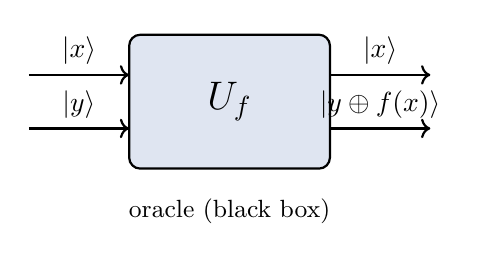
\begin{tikzpicture}[scale=0.85]
    \draw[thick, fill=circuitblue!15, rounded corners] (0, 0) rectangle (3, 2);
    \node[font=\Large] at (1.5, 1) {$U_f$};
    \draw[->, thick] (-1.5, 1.4) -- (0, 1.4) node[midway, above] {$\ket{x}$};
    \draw[->, thick] (-1.5, 0.6) -- (0, 0.6) node[midway, above] {$\ket{y}$};
    \draw[->, thick] (3, 1.4) -- (4.5, 1.4) node[midway, above] {$\ket{x}$};
    \draw[->, thick] (3, 0.6) -- (4.5, 0.6) node[midway, above] {$\ket{y \oplus f(x)}$};
    \node[below] at (1.5, -0.3) {\small oracle (black box)};
\end{tikzpicture}
\end{center}

\begin{intuition}
think of the oracle as a black box machine. u feed it an input, it gives u an output, and u r charged per query. the question is: how many queries do u need to figure out some property of $f$? classical computers query with one input at a time. quantum computers can query with a \textbf{superposition of all inputs simultaneously} --- thats where the speedup comes from.
\end{intuition}

\subsection{Phase Oracle}

theres an alternative oracle formulation thats super useful. if $f: \{0,1\}^n \to \{0,1\}$ (single-bit output), u can convert the standard oracle into a \textbf{phase oracle}:

\[
\boxed{O_f\ket{x} = (-1)^{f(x)}\ket{x}}
\]

how? set the ancilla to $\ket{-} = \frac{1}{\sqrt{2}}(\ket{0} - \ket{1})$:
\begin{align}
U_f\ket{x}\ket{-} &= \ket{x}\frac{1}{\sqrt{2}}(\ket{0 \oplus f(x)} - \ket{1 \oplus f(x)}) \\
&= (-1)^{f(x)}\ket{x}\ket{-}
\end{align}

the phase $(-1)^{f(x)}$ gets ``kicked back'' onto the input register, and the ancilla remains $\ket{-}$. this is the phase kickback trick from lecture 2 in action.

%% ========================================================
\section{Deutsch's Algorithm}
%% ========================================================

\subsection{The Problem}

given a function $f: \{0,1\} \to \{0,1\}$ (one bit to one bit), determine whether $f$ is \textbf{constant} ($f(0) = f(1)$) or \textbf{balanced} ($f(0) \neq f(1)$).

there r four possible functions:
\begin{center}
\begin{tabular}{c|c|c|c}
$x$ & $f_1$ (const 0) & $f_2$ (const 1) & $f_3$ (balanced) \\
\hline
0 & 0 & 1 & 0 \\
1 & 0 & 1 & 1
\end{tabular}
\hspace{0.5cm}
\begin{tabular}{c|c}
$x$ & $f_4$ (balanced) \\
\hline
0 & 1 \\
1 & 0
\end{tabular}
\end{center}

\textbf{classically:} u need 2 queries (evaluate $f(0)$ and $f(1)$, then compare).

\textbf{quantumly:} 1 query suffices.

\subsection{The Circuit}

\begin{center}
\begin{quantikz}
\lstick{$\ket{0}$} & \gate{H} & \gate[2]{U_f} & \gate{H} & \meter{} \\
\lstick{$\ket{1}$} & \gate{H} & & \qw & \qw
\end{quantikz}
\end{center}

\subsection{Step-by-Step Analysis}

\textbf{initial state:} $\ket{0}\ket{1}$

\textbf{after H on both qubits:}
\[
\ket{+}\ket{-} = \frac{1}{\sqrt{2}}(\ket{0} + \ket{1}) \cdot \frac{1}{\sqrt{2}}(\ket{0} - \ket{1})
\]

\textbf{after oracle $U_f$} (using phase kickback):
\[
\frac{1}{\sqrt{2}}((-1)^{f(0)}\ket{0} + (-1)^{f(1)}\ket{1})\ket{-}
\]

factor out $(-1)^{f(0)}$:
\[
(-1)^{f(0)} \frac{1}{\sqrt{2}}(\ket{0} + (-1)^{f(0) \oplus f(1)}\ket{1})\ket{-}
\]

now there r two cases:
\begin{itemize}
    \item if $f$ is constant: $f(0) \oplus f(1) = 0$, so the state is $\pm\ket{+}\ket{-}$
    \item if $f$ is balanced: $f(0) \oplus f(1) = 1$, so the state is $\pm\ket{-}\ket{-}$
\end{itemize}

\textbf{after H on first qubit:}
\begin{itemize}
    \item constant: $H\ket{+} = \ket{0}$ $\Rightarrow$ measure $\boxed{0}$
    \item balanced: $H\ket{-} = \ket{1}$ $\Rightarrow$ measure $\boxed{1}$
\end{itemize}

\begin{keypoint}
deutsch's algorithm determines whether $f$ is constant or balanced with just \textbf{1 query} to the oracle, compared to 2 classically. its only a factor-of-2 speedup, which is unimpressive. but the principle --- query in superposition, use interference to extract a global property --- generalizes to exponential speedups in the next algorithms.
\end{keypoint}

\subsection{Worked Example}

\begin{example}
let $f(0) = 0, f(1) = 1$ (balanced, $f(x) = x$, i.e., the identity function).

the oracle is $U_f\ket{x}\ket{y} = \ket{x}\ket{y \oplus x}$, which is just a CNOT gate.

\begin{center}
\begin{quantikz}
\lstick{$\ket{0}$} & \gate{H} & \ctrl{1} & \gate{H} & \meter{} \\
\lstick{$\ket{1}$} & \gate{H} & \targ{} & \qw & \qw
\end{quantikz}
\end{center}

trace through:
\begin{align}
\ket{01} &\xrightarrow{H \otimes H} \ket{+}\ket{-} \\
&\xrightarrow{\text{CNOT}} \frac{1}{\sqrt{2}}(\ket{0}\ket{-} + \ket{1}(X\ket{-})) = \frac{1}{\sqrt{2}}(\ket{0}\ket{-} - \ket{1}\ket{-}) = \ket{-}\ket{-} \\
&\xrightarrow{H \otimes I} \ket{1}\ket{-}
\end{align}

measure first qubit: get 1. conclusion: $f$ is balanced. correct!
\end{example}

%% ========================================================
\section{Deutsch-Jozsa Algorithm}
%% ========================================================

\subsection{The Problem}

this is the natural generalization of deutsch's problem to $n$ bits.

given $f: \{0,1\}^n \to \{0,1\}$ with the \textbf{promise} that $f$ is either:
\begin{itemize}
    \item \textbf{constant}: $f(x) = c$ for all $x$ (same output for every input)
    \item \textbf{balanced}: $f(x) = 0$ for exactly half the inputs and $f(x) = 1$ for the other half
\end{itemize}
determine which case it is.

\textbf{classically (deterministic):} in the worst case, u need to query $2^{n-1} + 1$ inputs. bcs even after seeing $2^{n-1}$ identical outputs, the function could still be balanced (the remaining half could all be different).

\textbf{classically (randomized):} with high probability, $O(1)$ random queries suffice. if u query a few random inputs and they all give the same output, its very likely constant. but theres always a small probability of error.

\textbf{quantumly:} exactly 1 query, deterministic. no error.

\subsection{The Circuit}

\begin{center}
\begin{quantikz}
\lstick{$\ket{0}^{\otimes n}$} & \gate{H^{\otimes n}} & \gate[2]{U_f} & \gate{H^{\otimes n}} & \meter{} \\
\lstick{$\ket{1}$} & \gate{H} & & \qw & \qw
\end{quantikz}
\end{center}

\subsection{Analysis}

\textbf{after first layer of hadamards:}
\[
\frac{1}{\sqrt{2^n}}\sum_{x=0}^{2^n-1}\ket{x} \otimes \ket{-}
\]

\textbf{after oracle} (phase kickback):
\[
\frac{1}{\sqrt{2^n}}\sum_{x=0}^{2^n-1}(-1)^{f(x)}\ket{x} \otimes \ket{-}
\]

\textbf{after second layer of hadamards} on the first register. we need the n-qubit hadamard identity:
\[
H^{\otimes n}\ket{x} = \frac{1}{\sqrt{2^n}}\sum_{y=0}^{2^n-1}(-1)^{x \cdot y}\ket{y}
\]
where $x \cdot y = \sum_i x_i y_i \pmod{2}$ is the bitwise inner product.

so:
\begin{align}
&\frac{1}{\sqrt{2^n}}\sum_x (-1)^{f(x)} \cdot \frac{1}{\sqrt{2^n}}\sum_y (-1)^{x \cdot y}\ket{y} \\
= &\sum_y \left[\frac{1}{2^n}\sum_x (-1)^{f(x) + x \cdot y}\right]\ket{y}
\end{align}

the amplitude of $\ket{0^n}$ (all zeros) is:
\[
\boxed{\alpha_{0^n} = \frac{1}{2^n}\sum_{x=0}^{2^n-1}(-1)^{f(x)}}
\]

\begin{itemize}
    \item if $f$ is constant: $\alpha_{0^n} = \frac{1}{2^n} \cdot (\pm 2^n) = \pm 1$. probability of measuring $\ket{0^n}$ is $\boxed{1}$.
    \item if $f$ is balanced: $\alpha_{0^n} = \frac{1}{2^n}(2^{n-1} \cdot 1 + 2^{n-1} \cdot (-1)) = 0$. probability of measuring $\ket{0^n}$ is $\boxed{0}$.
\end{itemize}

\begin{keypoint}
the algorithm: measure the first register. if u get $0^n$, the function is constant. if u get anything else, its balanced. one query, deterministic, no error. this is an \textbf{exponential speedup} over deterministic classical algorithms.
\end{keypoint}

\begin{intuition}
why does this work? the hadamard-oracle-hadamard structure creates interference. for a constant function, all the phases $(-1)^{f(x)}$ r the same, so they constructively interfere at $\ket{0^n}$. for a balanced function, half the phases r $+1$ and half r $-1$, so they perfectly cancel at $\ket{0^n}$ (destructive interference). the interference pattern encodes the global property (constant vs balanced) into a single measurement outcome.
\end{intuition}

\subsection{Oracle Construction Example}

\begin{example}
for $n = 2$, consider the balanced function $f(00) = 0, f(01) = 1, f(10) = 1, f(11) = 0$.

the phase oracle applies $(-1)^{f(x)}$:
\[
O_f = \text{diag}(1, -1, -1, 1)
\]

this can be decomposed as: $O_f = \text{CZ}_{12} \cdot (I \otimes Z)$ or equivalently using the fact that $(-1)^{x_1 \oplus x_2}$ where $f(x_1 x_2) = x_1 \oplus x_2$. the oracle is a CNOT followed by a Z on the second qubit (in the phase oracle formulation).

trace through the full algorithm:
\begin{align}
\ket{00} &\xrightarrow{H^{\otimes 2}} \frac{1}{2}(\ket{00} + \ket{01} + \ket{10} + \ket{11}) \\
&\xrightarrow{O_f} \frac{1}{2}(\ket{00} - \ket{01} - \ket{10} + \ket{11}) \\
&\xrightarrow{H^{\otimes 2}} \ket{11}
\end{align}

measure: $\ket{11} \neq \ket{00}$, so $f$ is balanced. correct!
\end{example}

%% ========================================================
\section{Bernstein-Vazirani Algorithm}
%% ========================================================

\subsection{The Problem}

given an oracle for $f: \{0,1\}^n \to \{0,1\}$ with the promise that $f(x) = s \cdot x \pmod{2}$ for some unknown ``secret string'' $s \in \{0,1\}^n$, find $s$.

here $s \cdot x = s_1 x_1 \oplus s_2 x_2 \oplus \cdots \oplus s_n x_n$ is the bitwise inner product mod 2.

\textbf{classically:} u need $n$ queries. query $f(e_i)$ for each standard basis vector $e_i = 00\ldots010\ldots0$ (1 in position $i$). then $f(e_i) = s_i$, revealing one bit of $s$ per query.

\textbf{quantumly:} 1 query.

\subsection{The Circuit}

the circuit is \textbf{identical} to deutsch-jozsa:

\begin{center}
\begin{quantikz}
\lstick{$\ket{0}^{\otimes n}$} & \gate{H^{\otimes n}} & \gate[2]{U_f} & \gate{H^{\otimes n}} & \meter{} \\
\lstick{$\ket{1}$} & \gate{H} & & \qw & \qw
\end{quantikz}
\end{center}

\subsection{Analysis}

after H, oracle (phase kickback), and H:
\[
\sum_y \left[\frac{1}{2^n}\sum_x (-1)^{s \cdot x + x \cdot y}\right]\ket{y} = \sum_y \left[\frac{1}{2^n}\sum_x (-1)^{x \cdot (s \oplus y)}\right]\ket{y}
\]

the inner sum is:
\[
\frac{1}{2^n}\sum_x (-1)^{x \cdot (s \oplus y)} = \begin{cases} 1 & \text{if } s \oplus y = 0^n \text{ (i.e., } y = s) \\ 0 & \text{otherwise} \end{cases}
\]

this uses the \textbf{hadamard identity}: $\sum_x (-1)^{x \cdot z} = 2^n \delta_{z, 0^n}$.

so the final state is simply $\ket{s}$. measure and u get the secret string directly.

\begin{keypoint}
bernstein-vazirani achieves an exponential speedup: 1 quantum query vs $n$ classical queries. the algorithm reveals \textbf{all $n$ bits of the secret string simultaneously} by querying the oracle with a superposition of all possible inputs.
\end{keypoint}

\begin{example}
$n = 3$, secret string $s = 101$.

$f(x) = x_1 \oplus x_3$ (inner product of $x$ with $101$).

the oracle adds a phase $(-1)^{x_1 \oplus x_3}$. after H-oracle-H:

final state: $\ket{101}$.

measure: $101$. we recover $s = 101$ in one shot.
\end{example}

%% ========================================================
\section{Simon's Algorithm}
%% ========================================================

\subsection{The Problem}

given an oracle for $f: \{0,1\}^n \to \{0,1\}^n$ with the promise that there exists a ``period'' $s \in \{0,1\}^n$ such that:
\[
f(x) = f(y) \iff x \oplus y \in \{0^n, s\}
\]

find $s$. (if $s = 0^n$, then $f$ is one-to-one. otherwise, $f$ is two-to-one.)

\textbf{classically:} requires $\Omega(2^{n/2})$ queries (birthday paradox argument).

\textbf{quantumly:} $O(n)$ queries and classical post-processing.

this is an \textbf{exponential speedup} --- the first problem where quantum computing provably offers an exponential advantage.

\subsection{The Circuit}

\begin{center}
\begin{quantikz}
\lstick{$\ket{0}^{\otimes n}$} & \gate{H^{\otimes n}} & \gate[2]{U_f} & \gate{H^{\otimes n}} & \meter{} \\
\lstick{$\ket{0}^{\otimes n}$} & \qw & & \qw & \qw
\end{quantikz}
\end{center}

\subsection{Analysis}

\textbf{after hadamards:}
\[
\frac{1}{\sqrt{2^n}}\sum_x \ket{x}\ket{0^n}
\]

\textbf{after oracle:}
\[
\frac{1}{\sqrt{2^n}}\sum_x \ket{x}\ket{f(x)}
\]

now, conceptually, suppose we measure the second register and get some value $f(z)$. then the first register collapses to a superposition of the (at most two) inputs that map to $f(z)$:

if $s \neq 0^n$:
\[
\frac{1}{\sqrt{2}}(\ket{z} + \ket{z \oplus s})
\]

\textbf{after hadamards on first register:}
\begin{align}
&\frac{1}{\sqrt{2}} \cdot \frac{1}{\sqrt{2^n}}\sum_y [(-1)^{y \cdot z} + (-1)^{y \cdot (z \oplus s)}]\ket{y} \\
= &\frac{1}{\sqrt{2}} \cdot \frac{1}{\sqrt{2^n}}\sum_y (-1)^{y \cdot z}[1 + (-1)^{y \cdot s}]\ket{y}
\end{align}

the factor $[1 + (-1)^{y \cdot s}]$ is:
\begin{itemize}
    \item $2$ if $y \cdot s = 0$
    \item $0$ if $y \cdot s = 1$
\end{itemize}

so we only measure $y$ values satisfying $\boxed{y \cdot s = 0 \pmod{2}}$.

\subsection{Classical Post-Processing}

each run of the circuit gives us one equation $y \cdot s = 0$. after $O(n)$ runs, we collect $n-1$ linearly independent equations and solve the linear system over $\mathbb{F}_2$ (binary field) to find $s$.

\begin{keypoint}
simon's algorithm structure:
\begin{enumerate}
    \item repeat $O(n)$ times: run the quantum circuit, measure, get a random $y$ satisfying $y \cdot s = 0$
    \item collect all the $y$ values into a matrix
    \item solve the null space to find $s$ (gaussian elimination over $\mathbb{F}_2$)
\end{enumerate}
total: $O(n)$ quantum queries + $O(n^3)$ classical post-processing. exponentially better than the $O(2^{n/2})$ classical query complexity.
\end{keypoint}

\begin{example}
$n = 3$, $s = 110$.

after several runs, suppose we collect:
\begin{align}
y_1 = 001: \quad 0 \cdot 1 + 0 \cdot 1 + 1 \cdot 0 &= 0 \quad \checkmark \\
y_2 = 110: \quad 1 \cdot 1 + 1 \cdot 1 + 0 \cdot 0 &= 0 \quad \checkmark \\
y_3 = 111: \quad 1 \cdot 1 + 1 \cdot 1 + 1 \cdot 0 &= 0 \quad \checkmark
\end{align}

we need to find $s$ such that $y_i \cdot s = 0$ for all $i$.

from the linear system (gaussian elimination): $s_1 = s_2$, $s_3 = 0$. nontrivial solution: $s = 110$.
\end{example}

\subsection{Why Simon's Algorithm Matters}

\begin{intuition}
simon's algorithm is historically important bcs it was the first to show an exponential quantum speedup for a well-defined problem. it directly inspired peter shor to develop his factoring algorithm, which is essentially a continuous version of simon's algorithm (replacing the XOR group structure with modular arithmetic).

the key insight from simon's algorithm: the hadamard transform converts the oracle's \textbf{domain structure} (the period $s$) into \textbf{linear constraints} on the measurement outcomes. this is a recurring theme in quantum algorithms.
\end{intuition}

%% ========================================================
\section{Comparison of the Algorithms}
%% ========================================================

\begin{center}
\begin{tabular}{l|c|c|c}
algorithm & problem & classical queries & quantum queries \\
\hline
deutsch & constant vs balanced ($n=1$) & 2 & 1 \\
deutsch-jozsa & constant vs balanced ($n$ bits) & $2^{n-1}+1$ & 1 \\
bernstein-vazirani & find secret string $s$ & $n$ & 1 \\
simon & find period $s$ & $\Omega(2^{n/2})$ & $O(n)$
\end{tabular}
\end{center}

\begin{keypoint}
all four algorithms share the same structure:
\begin{enumerate}
    \item hadamard: create superposition
    \item oracle: encode function information into phases
    \item hadamard: create interference
    \item measure: read out the answer
\end{enumerate}
the H-oracle-H sandwich is the fundamental quantum algorithm pattern. the difference between the algorithms is in the oracle structure and wt information the interference reveals.
\end{keypoint}

heres a visual of how the speedups scale:

\begin{center}
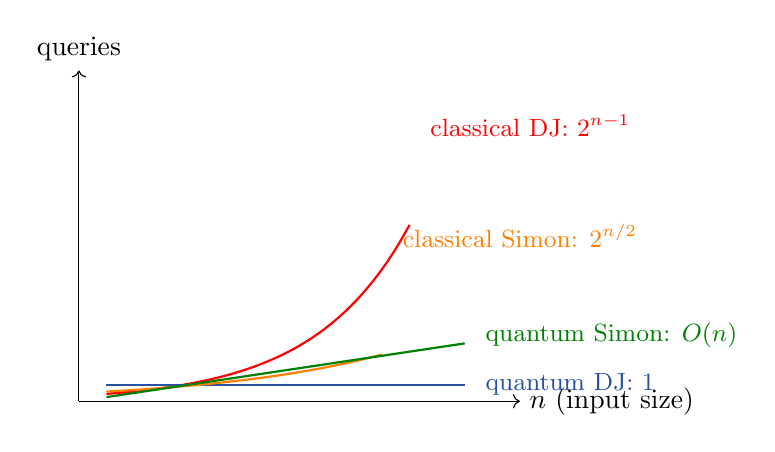
\begin{tikzpicture}[scale=0.7]
    \draw[->] (0,0) -- (8,0) node[right] {$n$ (input size)};
    \draw[->] (0,0) -- (0,6) node[above] {queries};

    % classical DJ
    \draw[thick, red, domain=0.5:6, smooth] plot (\x, {0.1*2^(\x/1.2)});
    \node[red, right] at (6.2, 5) {\small classical DJ: $2^{n-1}$};

    % quantum DJ
    \draw[thick, circuitblue] (0.5, 0.3) -- (7, 0.3);
    \node[circuitblue, right] at (7.2, 0.3) {\small quantum DJ: $1$};

    % classical simon
    \draw[thick, orange, domain=0.5:5.5, smooth] plot (\x, {0.15*2^(\x/2.2)});
    \node[orange, right] at (5.7, 3) {\small classical Simon: $2^{n/2}$};

    % quantum simon
    \draw[thick, green!50!black, domain=0.5:7] plot (\x, {0.15*\x});
    \node[green!50!black, right] at (7.2, 1.2) {\small quantum Simon: $O(n)$};
\end{tikzpicture}
\end{center}

deutsch-jozsa gives an exponential speedup (the most dramatic kind). simon gives a superpolynomial speedup. both use the same H-oracle-H sandwich --- the difference is in the oracle.

%% ========================================================
\section{The Hadamard Transform and Fourier Analysis}
%% ========================================================

the hadamard transform is doing smtg very specific: its the discrete fourier transform over $\mathbb{Z}_2^n$ (the group of $n$-bit binary strings under XOR).

\[
H^{\otimes n}\ket{x} = \frac{1}{\sqrt{2^n}}\sum_{y \in \{0,1\}^n} (-1)^{x \cdot y}\ket{y}
\]

this maps from the ``position basis'' to the ``frequency basis'' (just like the classical fourier transform). the oracle encodes information in the position basis, and the hadamard reveals the frequency-domain structure.

\begin{intuition}
the reason the H-oracle-H pattern works is bcs:
\begin{enumerate}
    \item first H: express the input as a superposition in the position basis
    \item oracle: the oracle modifies the amplitudes based on $f(x)$, encoding the function's structure into the position-basis amplitudes
    \item second H: fourier transform to the frequency basis, where the function's global properties (constant vs balanced, period, secret string) become directly readable from the amplitudes
\end{enumerate}
global properties of $f$ become \textbf{localized} in the fourier domain. this is the deep reason quantum algorithms work.
\end{intuition}

\subsection{The Boolean Fourier Expansion}

any boolean function $f: \{0,1\}^n \to \{-1, 1\}$ can be written as:
\[
f(x) = \sum_{S \subseteq [n]} \hat{f}(S) \chi_S(x)
\]
where $\chi_S(x) = (-1)^{\bigoplus_{i \in S} x_i}$ r the parity functions and $\hat{f}(S)$ r the fourier coefficients.

the deutsch-jozsa and bernstein-vazirani algorithms can be understood as measuring specific fourier coefficients of $f$ --- the quantum circuit is literally computing the fourier transform and reading off the coefficients.

%% ========================================================
\section{Detailed Worked Examples}
%% ========================================================

\subsection{Deutsch-Jozsa with $n = 3$}

\begin{example}
let $f: \{0,1\}^3 \to \{0,1\}$ be balanced, defined by $f(x) = x_1$ (output is just the first bit).

so $f(000) = 0, f(001) = 0, f(010) = 0, f(011) = 0, f(100) = 1, f(101) = 1, f(110) = 1, f(111) = 1$.

this is balanced: exactly 4 inputs give 0 and 4 inputs give 1.

the phase oracle: $O_f\ket{x_1 x_2 x_3} = (-1)^{x_1}\ket{x_1 x_2 x_3}$. this is just $Z \otimes I \otimes I$ acting on the first qubit.

\textbf{step 1:} $H^{\otimes 3}\ket{000} = \ket{+++}$

\textbf{step 2:} $(Z \otimes I \otimes I)\ket{+++} = \ket{-}\ket{+}\ket{+}$

(bcs $Z\ket{+} = \ket{-}$)

\textbf{step 3:} $H^{\otimes 3}\ket{-++} = \ket{1}\ket{0}\ket{0} = \ket{100}$

measure: $\ket{100} \neq \ket{000}$, so $f$ is balanced. correct!

note: the measurement outcome $100$ actually tells u that $f$ depends on $x_1$ --- the bernstein-vazirani algorithm extracts even more information from the same circuit.
\end{example}

\subsection{Bernstein-Vazirani with $n = 4$}

\begin{example}
secret string $s = 1011$.

$f(x) = x_1 \oplus x_3 \oplus x_4$ (inner product with $1011$).

the oracle applies phase $(-1)^{x_1 \oplus x_3 \oplus x_4}$:

$O_f = Z_1 \otimes I_2 \otimes Z_3 \otimes Z_4$

(each qubit position where $s_i = 1$ gets a Z gate).

the circuit: $H^{\otimes 4} \cdot O_f \cdot H^{\otimes 4}\ket{0000}$

$H^{\otimes 4}\ket{0000} = \ket{++++}$

$O_f\ket{++++} = Z_1\ket{+} \otimes \ket{+} \otimes Z_3\ket{+} \otimes Z_4\ket{+} = \ket{-}\ket{+}\ket{-}\ket{-}$

$H^{\otimes 4}\ket{-+-{-}} = \ket{1}\ket{0}\ket{1}\ket{1} = \ket{1011}$

measure: $1011 = s$. done in one query.
\end{example}

\subsection{Simon's Algorithm: Full 3-Qubit Example}

\begin{example}
let $n = 2$, $s = 11$.

define $f$ by: $f(00) = 01, f(01) = 10, f(10) = 10, f(11) = 01$.

check: $f(00) = f(11)$ and $00 \oplus 11 = 11 = s$. $f(01) = f(10)$ and $01 \oplus 10 = 11 = s$. good.

\textbf{run 1:}

$\ket{00}\ket{00} \xrightarrow{H^{\otimes 2} \otimes I} \frac{1}{2}(\ket{00} + \ket{01} + \ket{10} + \ket{11})\ket{00}$

$\xrightarrow{U_f} \frac{1}{2}(\ket{00}\ket{01} + \ket{01}\ket{10} + \ket{10}\ket{10} + \ket{11}\ket{01})$

$= \frac{1}{2}[(\ket{00} + \ket{11})\ket{01} + (\ket{01} + \ket{10})\ket{10}]$

if we measure the second register and get $\ket{01}$:

first register collapses to $\frac{1}{\sqrt{2}}(\ket{00} + \ket{11})$

$\xrightarrow{H^{\otimes 2}} \frac{1}{\sqrt{2}}(\ket{++} + \ket{--})$

$= \frac{1}{\sqrt{2}} \cdot \frac{1}{2}[(\ket{00} + \ket{01} + \ket{10} + \ket{11}) + (\ket{00} - \ket{01} - \ket{10} + \ket{11})]$

$= \frac{1}{\sqrt{2}}(\ket{00} + \ket{11})$

measure: get either $00$ or $11$, each with probability $1/2$.

if we get $y = 11$: check $y \cdot s = 1 \cdot 1 + 1 \cdot 1 = 0 \pmod{2}$. $\checkmark$

if we get $y = 00$: trivially $y \cdot s = 0$. (uninformative, need another run)

after enough runs collecting nontrivial $y$ values, we solve to find $s = 11$.
\end{example}

%% ========================================================
\section{Limitations and Context}
%% ========================================================

\begin{keypoint}
important caveats:
\begin{itemize}
    \item these algorithms work in the \textbf{oracle model} --- the speedup is relative to oracle queries, not total computation time
    \item in practice, constructing the oracle itself might require exponential resources, which would negate the query advantage
    \item deutsch-jozsa solves a problem that doesnt arise naturally in practice
    \item the randomized classical algorithm for deutsch-jozsa needs only $O(1)$ queries with bounded error --- so the quantum advantage is only over \textbf{deterministic} classical algorithms
    \item simon's algorithm inspired shor's algorithm, which DOES solve a practically important problem (factoring)
    \item the techniques --- superposition, interference, phase kickback, fourier analysis --- show up everywhere in quantum computing
\end{itemize}
\end{keypoint}

%% ========================================================
\section{Summary}
%% ========================================================

\begin{keypoint}
wt to remember from this lecture:
\begin{enumerate}
    \item the H-oracle-H sandwich is the fundamental pattern of quantum algorithms
    \item phase kickback converts oracle queries into phase information
    \item interference amplifies correct answers and cancels wrong ones
    \item deutsch: constant vs balanced, 1 qubit, 1 query
    \item deutsch-jozsa: constant vs balanced, $n$ qubits, 1 query
    \item bernstein-vazirani: find secret string, 1 query
    \item simon's: find period, $O(n)$ queries (exponential speedup)
    \item the hadamard transform is the fourier transform over $\mathbb{Z}_2^n$ --- this is the mathematical reason these algorithms work
\end{enumerate}
\end{keypoint}

next up: QFT, phase estimation, shor's algorithm, and grover's search. these take the same principles and apply them to much more powerful settings.

\end{document}
